% 115 120
\documentclass[12pt,a4paper]{amsart}
% ukazi za delo s slovenscino -- izberi kodiranje, ki ti ustreza
\usepackage[slovene]{babel}
%\usepackage[cp1250]{inputenc}
%\usepackage[T1]{fontenc}
\usepackage[utf8]{inputenc}
\usepackage{amsmath,amssymb,amsfonts}
\usepackage{url}
%\usepackage[normalem]{ulem}
\usepackage[dvipsnames,usenames]{color}
\usepackage{graphicx}

% ne spreminjaj podatkov, ki vplivajo na obliko strani
\textwidth 15cm
\textheight 24cm
\oddsidemargin.5cm
\evensidemargin.5cm
\topmargin-5mm
\addtolength{\footskip}{10pt}
\pagestyle{plain}
\overfullrule=15pt % oznaci predlogo vrstico


% ukazi za matematicna okolja
\theoremstyle{definition} % tekst napisan pokoncno
\newtheorem{definicija}{Definicija}[section]
\newtheorem{primer}[definicija]{Primer}
\newtheorem{opomba}[definicija]{Opomba}

\renewcommand\endprimer{\hfill$\diamondsuit$}


\theoremstyle{plain} % tekst napisan posevno
\newtheorem{lema}[definicija]{Lema}
\newtheorem{izrek}[definicija]{Izrek}
\newtheorem{trditev}[definicija]{Trditev}
\newtheorem{posledica}[definicija]{Posledica}


% za stevilske mnozice uporabi naslednje simbole
\newcommand{\R}{\mathbb R}
\newcommand{\N}{\mathbb N}
\newcommand{\Z}{\mathbb Z}
\newcommand{\C}{\mathbb C}
\newcommand{\Q}{\mathbb Q}


% ukaz za slovarsko geslo
\newlength{\odstavek}
\setlength{\odstavek}{\parindent}
\newcommand{\geslo}[2]{\noindent\textbf{#1}\hspace*{3mm}\hangindent=\parindent\hangafter=1 #2}


% naslednje ukaze ustrezno popravi
\newcommand{\program}{Finančna matematika} % ime studijskega programa: Matematika/Finan"cna matematika
\newcommand{\imeavtorja}{Martin Praček in Mela Malej} % ime avtorja
\newcommand{\imementorja}{Riste Škrekovski} % akademski naziv in ime mentorja
\newcommand{\naslovdela}{Graffiti Conjecture 194}
\newcommand{\letnica}{2019} %letnica diplome


% vstavi svoje definicije ...




\begin{document}
	
	% od tod do povzetka ne spreminjaj nicesar
	\thispagestyle{empty}
	\noindent{\large
		UNIVERZA V LJUBLJANI\\[1mm]
		FAKULTETA ZA MATEMATIKO IN FIZIKO\\[5mm]
		\program\ -- 1.~stopnja}
	\vfill
	
	\begin{center}{\large
			\imeavtorja\\[2mm]
			{\bf \naslovdela}\\[10mm]
			Seminarska naloga\\[1cm]
			Mentor: \imementorja}
	\end{center}
	\vfill
	
	\noindent{\large
		Ljubljana, \letnica}
	\pagebreak
	
	\thispagestyle{empty}
	\tableofcontents
	\pagebreak
	
	\thispagestyle{empty}
	\begin{center}
		{\bf \naslovdela}\\[3mm]
		{\sc Povzetek}
		\ \\
		Za predmet Finančni praktikum v študijskem letu $2018/19$ Martin Praček in Mela Malej dobila nalogo predstaviti problem Grafittijeve konjekuture $194$. \\
		To nalogo sva naredila s splošno kodo ter genetskim algoritmom.\\
		
	\end{center}

\pagebreak
\section{Predstavitev problema}
Grafittijeva konjektura 194 nam zastavi vprašanje iz teorije grafov.Zanima nas, ali za vsak preprost, povezan graf, ki zadošča pogoju $$ \alpha(G) \leq 1 + \lambda_{avg}(G),$$ velja, da obstaja hamiltonska pot. Gre za računalniško generirano trditev, pri kateri nas zanima, ali lahko najdemo protiprimer, kar je tudi najina glavna naloga.\\
\section{Pogoji našega problema}
Naš pogoj je torej 
\ \\
$$ \alpha(G) \leq 1 + \lambda_{avg}(G),$$
\ \\
kjer je $G$ naš graf, $\alpha(G)$ je neodvisnostno število, $\lambda_{avg}$ pa je povprečna lokalna neodvisnost grafa.\\
\ \\
\textbf{Neodvistnostno število grafa} $\alpha(G)$ nam pove moč največje množice, ki vsebuje  vozlišča grafa $G$, od katerih nobeni dve niste sosednji.\\
\ \\
\textbf{Lokalna neodvistnost grafa} $\lambda(G, v)$ nam pove neodvistnostno število podgrafa $Gv$ grafa $G$, kjer je $Gv$ definiran na sosedih vozlišča $v$. $\lambda_{avg}(G)$ nam pove povprečno lokalno neodvistnost.\\
\begin{figure}[h]
	\centering

	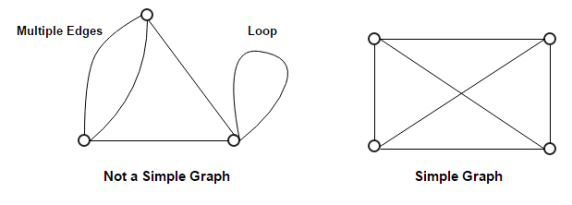
\includegraphics[scale=1]{slike/graf1}
\end{figure}

Ves čas zahtevamo, da je graf \textbf{preprost in povezan}. Ta zahteva pomeni, da ne obstaja vozlišče, ki ne bi bilo sosednje vsaj enemu drugemu vozlišču,  med dvema povezavama obstaja kvečjemu ena povezava, poleg tega pa ne obstaja  povezava od vozlišča $v$ do vozlišča $v$, kar pomeni da ne obstajajo zanke na enem vozlišču.\\
 
Graf ima \textbf{hamiltonsko pot}, če obstajata dve vozlišči, ki ju povezuje pot, ki natančno enkrat obišče vsako vozlišče grafa.\\
\ \\
Najina naloga je torej na dovolj velikem vzorcu grafov pokazati da to velja, ali pa dobiti protiprimer, ki bo dokazal da to ne drži.\\
\subsection{Primer}
Za lažje razumevanje je tukaj še poseben primer, ki mu moramo določiti neodvisnostno število ter povprečno lokalno neodvisnost.\\
\begin{figure}[h]
	\centering
	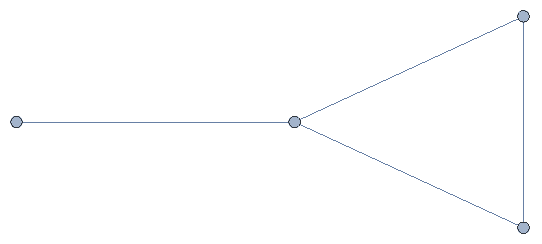
\includegraphics{slike/grafek}
\end{figure}
\\
\\
Očitno je neodvistnostno število $2$, povprečna lokalna neodvistnost pa je\\ $$\frac{1+3+1+1}{4}=\frac{6}{4}.$$
\ \\
Naša neenakost torej pravi, da je $$2 \leq 1+ \frac{6}{4},$$ 
\\kar drži. Naša naloga sedaj je dokazati, da hamiltonska pot ne obstaja. Vendar nam to v našem primeru ne bo uspelo, saj jo lahko precej enostavno najdemo.
\section{Delo}
Z najinim delom sva pričela v programskem jeziku Python, vendar sva hitro ugotovila sizifovstvo tega početja, in vse prestavila v programski jezik Sage, kjer sva v CoCalc spisala najino kodo v Jupyter Notebook. \\
\section{Koda in ideja programa}
Glavna ideja najine kode sledi glavni ideji najine naloge. Po vrsti sva razvrstila vse koščke neenakosti, in nato pogledala, če za primerne grafe le ta tudi velja. Tako sva dobila vrsto pomožnih ter eno glavno funkcijo.
\subsection{Pomožne funkcije}
Kot že rečeno, sva v okvirju najinega dela uporabila vrsto pomožnih funkcij. 
\subsubsection{neodvistnostno\_stevilo(G)}
Ta funkcija nam vrne neodvistnostno število grafa G. Tukaj smo si pomagali z funkcijo $.independent\_set()$, ki vrne največjo množico, kjer nobeni vozlišči nista sosednji.s 
\begin{figure}
	\includegraphics[scale=0.7]{slike/neodvisnost}
\end{figure}
\ \\


\subsubsection{lokalna\_neodvistnost(G, vozlisce)}
Ta funkcija nam vrne lokalno neodvistnost grafa G.
\begin{figure}
	\includegraphics[scale=0.7]{slike/lokalna}
\end{figure}
\ \\


\subsubsection{povprecna(G)}
Ta funkcija nam vrne povprečno lokalno neodvisnost.
\begin{figure}
	\includegraphics[scale=0.7]{slike/povprecna}
\end{figure}
\ \\

\subsection{Glavna funkcija}
Glavna funkcija, s katero smo izvajali teste, je tako dobila končen izgled.
\begin{figure}
	\includegraphics[scale=0.7]{slike/preveri}
\end{figure}
\ \\


Na ta način smo oblikovali funkcije, s katerimi smo testirali grafe. Za večje število testov smo uporabili genetski algoritem.
\subsection{Genetski algoritem}

Genetski algoritem je vrsta algoritma, ki temelji na Darwinovi ideji o razvoju vrst in preživetju najmočnejših. Zelo pomembno pa je, kako določimo, kdo je tu najmočnejši, zato se moramo primerno odločiti za kriterij, po katerem bomo to delali. V našem primeru smo se odločili za čim manjše neodvisnostno število.\\

V našem primeru sva se odločila, da bo populacija rasla iz $zacetne\_populacija(maksimalna)$, kjer določimo začetno množico povezanih grafov. Z vrednostjo maksimalna smo določili največjo velikost generacije.\\
Nato sva te grafe razvrstila po določenem kriteriju in določila možnosti mutacije "populacije", torej vsakega izmed grafov. Grafu lahko dodamo ali odstranimo povezavo in dodamo ali odstranimo vozlišče, na koncu pa jih lahko še križamo.\\
Ko sva to naredila, sva najin genetski algoritem testirala.\\
\begin{figure}[h]
	\includegraphics{slike/cocalc2}
\end{figure}
\ \\
Test sva naredila na $10000$ generacijah, ki so bile lahko velike največ $10000$. Ker nam ta test ni vrnil izjeme predvidevava, da izjeme ni možno najti.\\
\ \\
Ker nas poleg uspešnosti kode navadno zanima tudi njena hitrost oziroma časovna zahtevnost, sva se tudi to odločila testirati. Odločila sva se za 
\end{document}